%=========================================================================
% (c) 2011, 2012 Josef Lusticky

\section{Network communication}
Thanks to uIP, described in section~\ref{sec:contiki-uip},
the network communication is not a matter for Contiki OS.
% 1 - see implementation/communication.tex
A problem might be a possible packet loss when communication uses UDP on transport layer.
The reason why this can happen often is explained in section~\ref{sec:contiki-uip}.
% 2
In NTP unicast mode, the packet loss might occur either for client's query to server
or for server's response to client.
If the client's query loss occurs, no server response will be sent.
Similarly, if the server's response loss occurs, no message will be received by the client.
Not to block a whole system till the response arrives
is therefore a desired behaviour of the client.

--- to design.tex ?
The AVR Raven platform features 802.15.4 support.
Contiki is used in conjunction with RZ USB Stick - 6LoWPAN.

The 6LoWPAN Adaptation Layer % see Interconnecting smart objects with IP
% IEEE 802.15.4
as RFC~4944 written by 6lowpan working group of IETF
made the underlaying IEEE 802.15.4 layer
look like an IPv6 link~\cite{6lowpan} and
\begin{figure}
  \centering
  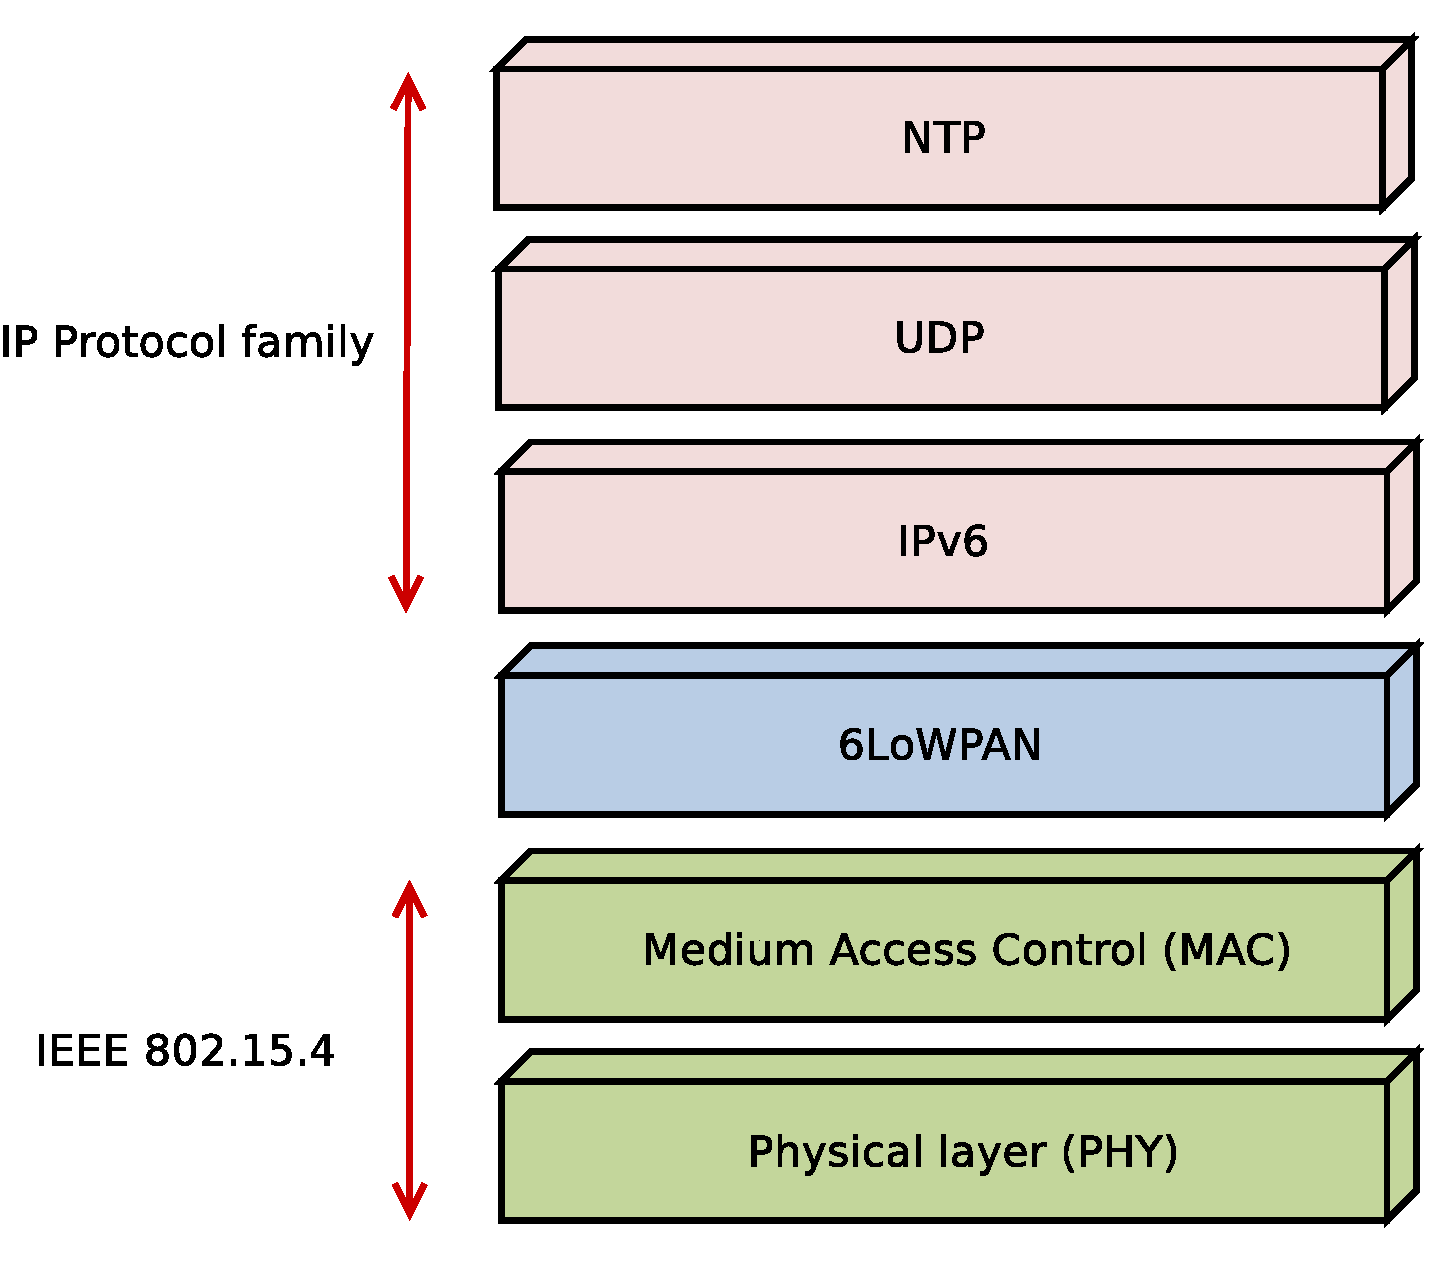
\includegraphics[width=9cm,keepaspectratio]{fig/6lowpan.pdf}
  \caption{Communication stack with 6lowpan layer}
  \label{fig:design-6lowpan}
  \bigskip
\end{figure}


Contiki supports broadcast packets as well as sending multicast packets.
Joining multicast groups through Internet Group Management Protocol (IGMP)
and receiving non-local multicast packets
was not supported at the time of writing~\cite{contiki-docs}.
Contiki is also able to use Domain Name System for IPv4 address resolution.
DNS resolution of IPv6 addresses was not implemented in Contiki OS
at the time of writing~\cite{contiki-docs}.
